%!TEX root = ../MasterThesis.tex

\section{Peer-to-peer communication}
\label{sec:p2p_communication}

This section explains the core concepts of \gls{P2P} communication technologies. It begins with a comparision of the benefits and disadvantages of centralized and decentralized Web architectures. After that it shows how \gls{P2P} communication networks can be structured, different ways to initiate a communication session as well as how data can be transmitted between peers.

\subsection{Centralized vs. Decentralized Web Architectures}
\label{sec:central_decentral_arch}

In classical client-server applications the information is stored on a central system (aka server). Clients have to connect to the server and ask for the information. The server handles the requests from the client and deliver the information in case the request was valid. A prominent example of the client-server architecture is the World-Wide Web as it exists today, in which clients (in this case the Web browser running on a computer) is communicating with a Web server (running on a server of the Web site provider) to access and retrieve Web documents (e.g.\ \gls{HTML}, images, audio, video, \ldots) transmitted via the \gls{HTTP} protocol, as shown in Figure~\ref{fig:p2p_central_server}. \@

\begin{figure}[H]
	\centering
		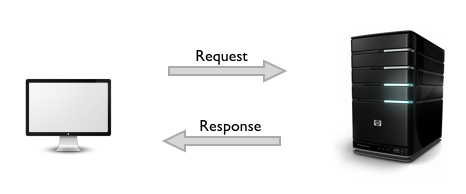
\includegraphics[width=0.9\columnwidth]{images/client-server-web.png}
	\caption[Client-Server communication used on the World-Wide Web]{Client-Server communication used on the World-Wide Web \citep{codeTuts}}
\label{fig:p2p_central_server}
\end{figure}

As a consequence of this architecture the information is centralized and under control of the provider of the (Web) server. This can lead to a variety of problems, e.g.\ unreliable or no longer existing servers will result in a dismissal of all the information stored on them, or privacy concerns for user-generated content stored on those central servers. \\

In opposite to that a \gls{P2P} network considers all nodes as equal. This offers the benefit that information can be kept on each node, and each node can provide access to its information to any other node on the network. Due to this the \gls{P2P} system has an high degree of decentralization, is not owned and controlled by a specific company, and therefore tends to me more resilient to faults, outages and attacks. But due to the distributed nature of it looking for and accessing information is more difficult. Information in a \gls{P2P} system have to be indexed in a way so that the correct node is queried for it. Still this index has to be stored somewhere in the system, and the optimal solution for the indexing problem depends on the type of \gls{P2P} system used (see next section). Additionally, the way new nodes get connected to the system is depending on the type of \gls{P2P} system used, and might lead to the introduction of special bootstrap or super nodes into the system as shown in Figure~\ref{fig:p2p_overlay_network} \citep{parameswaran2001p2p}.

\begin{figure}[H]
	\centering
		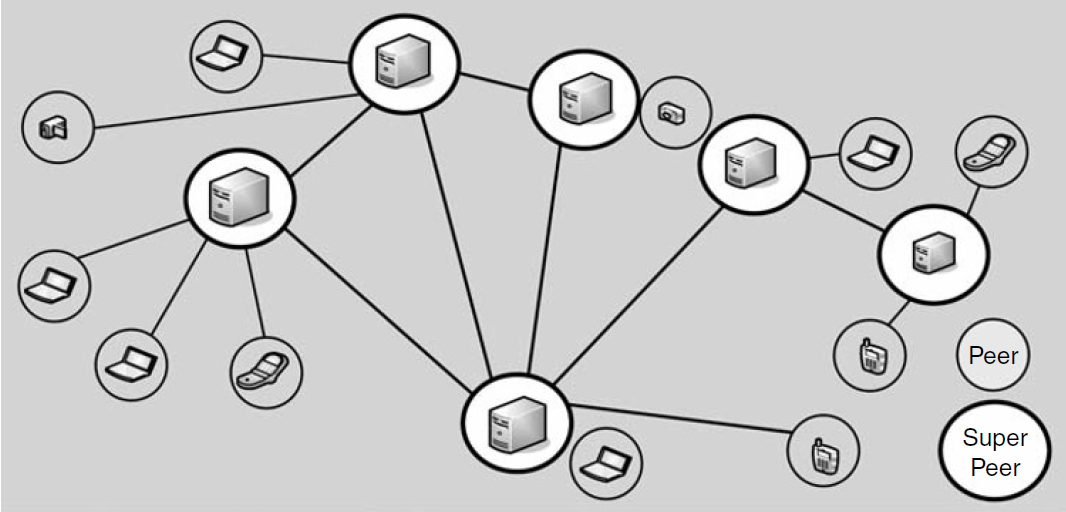
\includegraphics[width=0.9\columnwidth]{images/p2p_network.png}
	\caption[A \gls{P2P} overlay network]{A \gls{P2P} overlay network \citep[pg. 9]{buford2009p2p}}
\label{fig:p2p_overlay_network}
\end{figure}

% section central_decentral_arch (end)

\subsection{Classification of \gls{P2P} systems}
\label{sec:p2p_classification}

- can be categorized by the degree of centralization into: \\
1) partly centralized P2P systems (have a dedicated controller node that maintains the set of participating nodes and controls the system) \\
2) decentralized P2P systems (there are no dedicated nodes that are critical for the system operation) \\
- depends on the structure of the P2P system
- in a partly centralized P2P system new nodes join the network by connecting to the central controller (wellknown IP address) \\
- in a decentralized P2P system new nodes are expected to obtain via a separate channel the IP address to connect to (usually a bootstrap node that helps to set up the new node) \\
\\

% section p2p_init_session (end)

\subsection{Initiating a \gls{P2P} communication}
\label{sec:p2p_start_communication}

- also known as the overlay network in a P2P system \\
- can be represented as a directed graph containing the nodes and communication links between them \\
- can be differentiated between unstructured and structured overlays \\
- unstructured overlay networks have no constraints for the links between nodes; therefore the network has no particular structure \\
- structured overlay networks assign an unique identifier from a numeric keyspace to each node; these keys are used to assign certain responsibilities to nodes
on the network; as of this routing can be handled more efficiently \\
- in partly centralized P2P systems the controller is responsible for the overlay formation \\
\\
- in partly centralized P2P system an object is typically stored at the node that inserted the object \\
- the central controller holds the information about which objects exist and which nodes hold them \\
\\
- in unstructured systems the information is typically stored on the nodes that introduces them \\
- to locate an object a query request is typically broadcasted through the overlay network \\
- often the scope of the request (e.g. the maximum number of hops from the querying node forward) is limited to reduce the overhead on the system \\
\\
- in structured systems a distributed index is maintained in the form of a distributed hash table \\
- this DHT holds the hash value of the (index) key and the address of the node that stores the value \\
\\

% section p2p_start_communication

\subsection{The \gls{WebRTC} protocol}
\label{sec:p2p_webrtc}


% section p2p_webrtc (end)

% section p2p_communication (end)
